

\documentclass[final,a4paper,oneside,12pt]{article}
\setlength{\parindent}{0in}
 \usepackage{verbatim}
\usepackage{amsfonts}
\usepackage{amsmath}
\usepackage{color}
\usepackage{amssymb}
\usepackage[pdftex]{graphicx}
\begin{comment}
\usepackage[OT2,T1]{fontenc}
\DeclareSymbolFont{cyrletters}{OT2}{wncyr}{m}{n}
\DeclareMathSymbol{\Sha}{\mathalpha}{cyrletters}{"58}
\end{comment}
\usepackage{geometry}
%% Alex's thing
\setlength{\parskip}{0pt}
\setlength{\parsep}{0pt}
\setlength{\headsep}{0pt}
\setlength{\topskip}{0pt}
\setlength{\topmargin}{0pt}
\setlength{\topsep}{0pt}
\setlength{\partopsep}{0pt}
\linespread{1}

\geometry{
  body={7in, 10in},
  left=0.6in,
  top=0.5in
}

\setlength\parindent{0em}

\usepackage[compact]{titlesec}
\titlespacing{\section}{0pt}{*1}{*1}
\titlespacing{\subsection}{1pt}{*0.8}{*0.8}
\titlespacing{\subsubsection}{0pt}{*0}{*0}

\usepackage{amsfonts}
\usepackage{amsmath}
\usepackage{amssymb}
\usepackage[pdftex]{graphicx}
\usepackage{fullpage}
%%%
\begin{document}

\centerline{\Large \bf{Iron Concentration Plotter User Manual}}
\bigskip
\centerline{James McMurray}
\bigskip

\renewcommand{\labelenumi}{{\color{red} {\bf\arabic{enumi}}}}

\section{QSSPC Measurements}

\subsection{GUI Map}

When the program is first loaded the default tab is the ``QSSPC'' tab. Figure \ref{figure1} shows this window labelled when in use.

\begin{figure}[h]
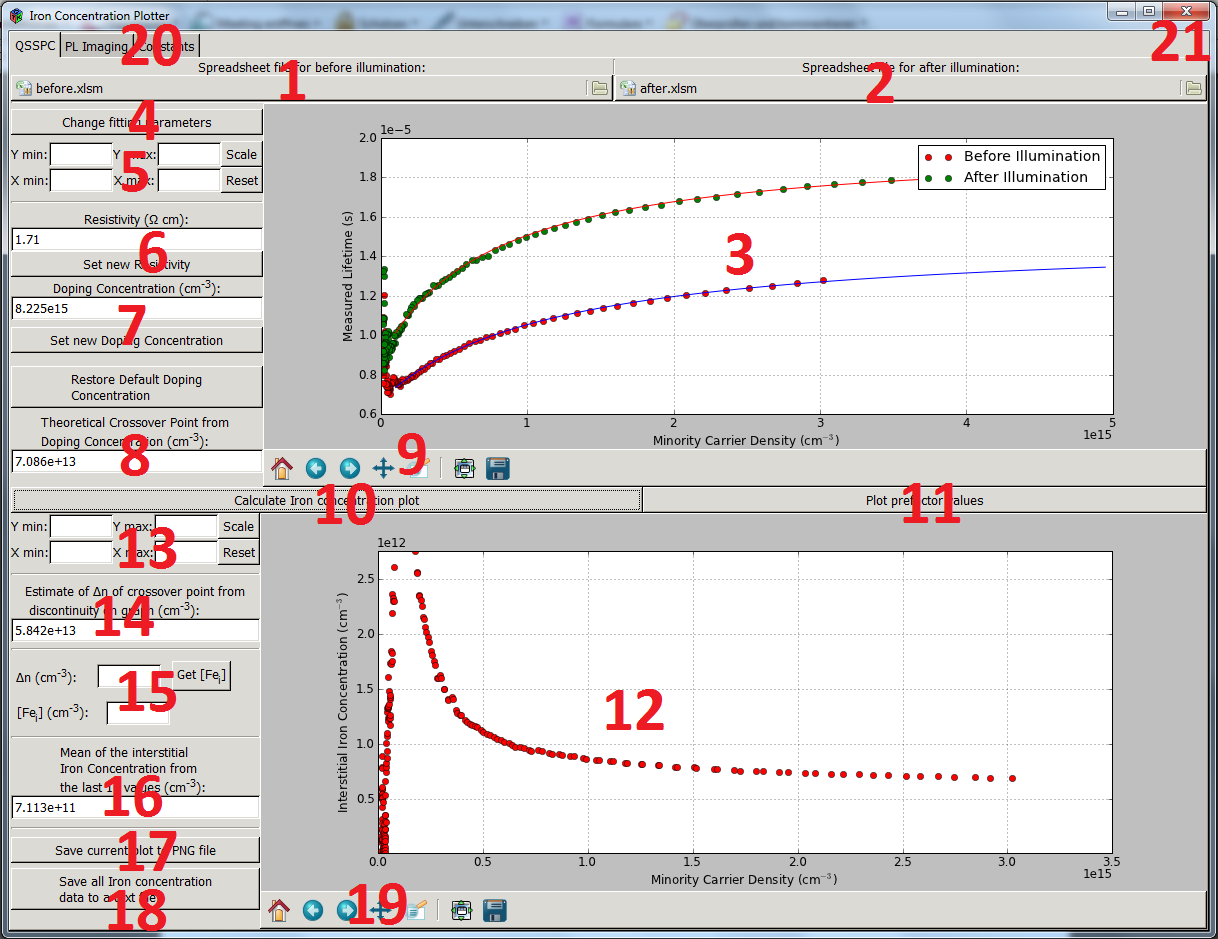
\includegraphics[height=5in]{2mainscreen}
\caption{\label{figure1} The QSSPC tab shown after loading the Excel files and plotting the graph of interstitial Iron Concentration.}
\end{figure}

\begin{enumerate}
\item The button used to load the Excel file for before illumination. The file loaded must be of .XLSM format and the program will check it can be loaded correctly.

\item The button used to load the Excel file for after illumination.

\item The area where the lifetime against injection level graphs (QSSPC measurements) are plotted from the Excel files. Hovering over it will give the X and Y values in the navigation toolbar below.

\item This button opens a window where the initial guess for the fits can be changed and the actual parameters plotted viewed.

\item Text boxes where the view window of the graph can be manually set. The numbers can be edited as they are on the graph i.e. X minimum as 1 and X maximum as 2, rather than 1e15 and 2e15 respectively, this is useful when zooming. However, this can occasionally cause problems (especially with graphs which have negative values), at which point the full specification with the exponent should be used. One box can be edited individually to change one part of the scale independently of the others.

\item  Here the Resistivity is read from the Excel file, and the Doping Concentration is calculated from it. The Resistivity value may be edited and the ``Set new Resistivity'' button used to set it and calculate the new Doping Concentration.

\item Here the calculated Doping Concentration is printed. The Doping Concentration may then be edited here to override the calculated value for calculating the interstitial Iron Concentration graph and the Photo-Luminescence (PL) maps.

\item Here a theoretical value is calculated for the Cross-Over Point (COP) from the Doping Concentration value using the equation given in Birkholz \textit{et al.} JAPL {\bf 97}, 103708 (2005)

\item The navigation toolbar for the QSSPC graph. The home button resets the view to default, or to the manually set value using the manual controls marked at {\color{red}{\bf 5}}. The back and forward buttons move between views that the user has set using the pan or zoom tool, like the Back/Forward buttons in a Web Browser, it does not pan itself. The panning tool pans across the graph by holding the leftm mouse button on the graph and dragging the mouse cursor in the opposite direction to the panning. The Zoom tool allows the user to click and draw a rectangle on the graph to zoom to. The Configure Subplots button adjusts the borders of the plot, this may be useful when saving. The save button allows the current plot to be saved.

\item This button calculates and plots the Iron Concentration graph.

\item This button calculates and plots the Prefactor values graph. It also changes controls {\color{red} {\bf 13}}, {\color{red} {\bf 14}}, {\color{red} {\bf 15}} and {\color{red} {\bf 16}} to work for the Prefactor values.

\item This is the area where the Iron Concentration plot is loaded. It behaves the same as the lifetime plot.

\item This is the area where the view can be set manually for the Iron Concentration/Prefactor values plot, it behaves the same as {\color{red} {\bf 5}}.

\item Here the COP is calculated from the graph as the point between the maximum Iron Concentration value and the next value (as the Iron Concentration tends to infinity at the COP).

\item Here a value for the injection level can be entered and the interstitial iron concentration value at this point will be printed.

\item Here the mean value of the last 10 values (i.e. highest injection level, so stable) of either the Iron Concentration or Prefactor values will be printed (depending on which graph is the actively plotted one).

\item This button saves the current plot to a PNG file, it is identical to the button in the navigation toolbars except it only supports PNG files.

\item This button saves the iron concentration plot data to a text file.

\item The Navigation Toolbar for the Iron Concentration graph. This behaves the same way as {\color{red} {\bf 9}}.

\item Here the other tabs can be opened for the PL Imaging and modifying the constants used in all calculations.

\item Here the application can be closed, maximised or minimised.
\end{enumerate}

\subsection{Usage}
The Excel files are loaded using the two buttons at the top of the screen and the QSSPC lifetime data is plotted. The doping concentration can then be changed manually if desired. The interstitial Iron Concentration against injection level plot can then be calculated and plotted, as can the prefactor values against injection levels.

\section{PL Imaging}
\subsection{GUI Map}

\begin{figure}[h]
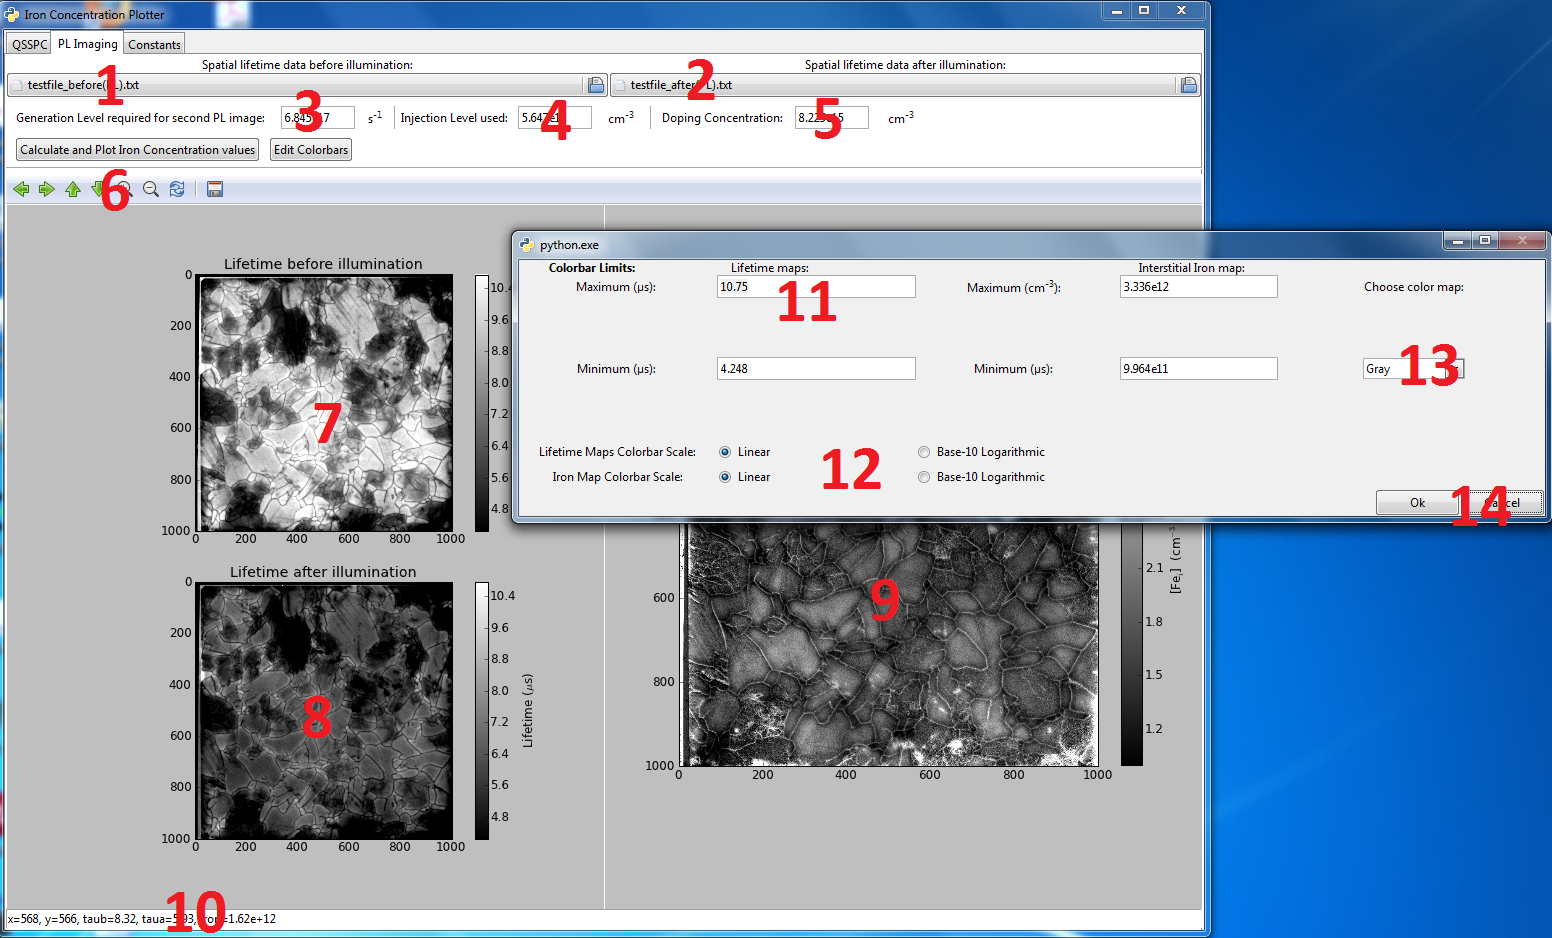
\includegraphics[height=4in]{pllabel}
\caption{\label{figure2} The PL imaging tab shown after loading the PL data files and plotting the PL maps for lifetime and interstitial iron concentration.The ``Edit Colorbars'' is also shown.}
\end{figure}

\begin{enumerate}
\item Here the PL data file for before illumination is selected. After selection a box will appear asking for the generation level used for this PL image, to determine the generation level required for the second PL image from the Excel files loaded in the QSSPC page.
\item Here the PL data file for after illumination is selected, the selection window lists the required generation level in the window title so it is easily viewable.
\item  Here the desired Generation Level for the after illumation PL data is listed so it can be read whilst selecting the file.
\item Here the injection level used in the calculation of the Iron Concentration PL Map is shown, and may be edited. It is read from the injection level corresponding to the given generation level in the Before Illumination Excel file.
\item Here is the Doping Concentration level, it is read from the Excel file and will be updated if it is changed on the QSSPC page. It can also be edited here for producing the PL maps.
\item The navigation toolbar, here the arrows are panning buttons, and the panning moves all the maps together to keep them comparable. The zooming function also works this way. The save button opens a dialog asking which plot or data to save.
\item The plot area for the before illumination lifetime map.
\item The plot area for the after illumination lifetime map. Note that both lifetime maps actually belong to the same figure, and so are saved together.
\item The plot area for the interstitial iron concentration map. Note that the iron concentration map is a separate figure from the lifetime figure and so must be saved separately.
\item The status bar, hovering over the plots provides details of the points here.
\item Here the limits to the colorbars can be changed.
\item Here the PL map colorbars can be set to use logarithmic scales.
\item Here the colormap can be changed.
\item Here the options are confirmed or cancelled. They only take effect if confirmed.
\end{enumerate}

\subsection{Usage}
Firstly the Excel files in the QSSPC page must be loaded. Then the PL before illumination data file can be selected, and the generation level used can be entered in to the dialog box. The PL after file is then chosen with the generation level closest to that given in the marked textbox and dialog title. The PL maps may then be calculated and plotted. The Iron Concentration map data can be saved under the save dialog after clicking the save icon in the toolbar.
\pagebreak
\section{Editing Constants}
\subsection{GUI Map}
\begin{figure}[h!]
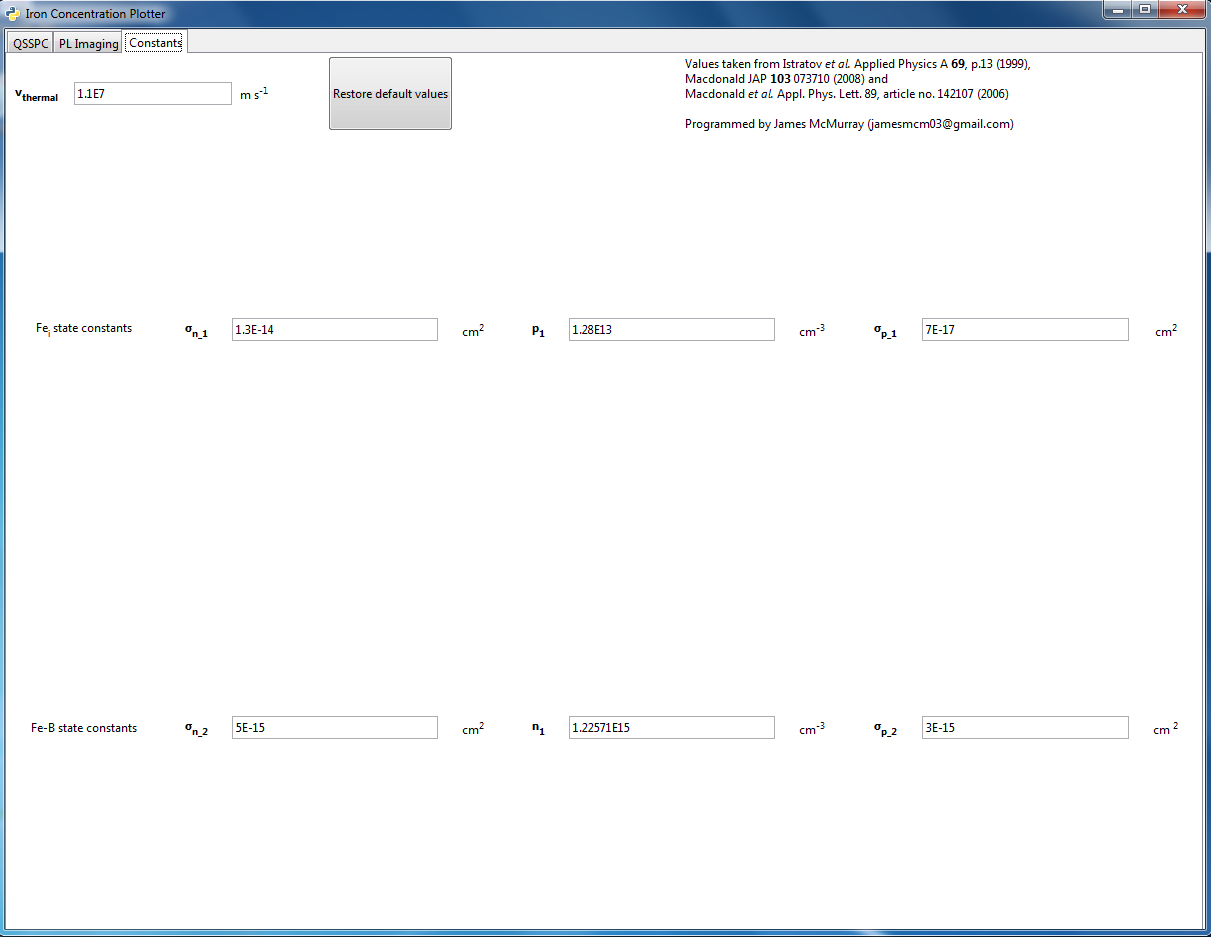
\includegraphics[height=5in]{constants}
\caption{\label{figure3} The Constants tab, here the constants can be edited.}
\end{figure}

\subsection{Usage}
Here the constants can be edited and their default values restored via the ``Restore Default Values'' button. The modified constants will take effect whenever there is a next calculation, so if you wish to apply them you will need to recalculate what has already been calculated (i.e. the PL maps or the QSSPC Iron Concentration plot).
\end{document}







